\documentclass{beamer}

\usetheme{Madrid}
\usecolortheme{default}

\usepackage{tikz}
\usetikzlibrary{shapes,arrows,positioning,automata}
\usepackage{amsmath}
\usepackage{amssymb}
\usepackage{listings}
\usepackage{graphicx}
\usepackage[T1]{fontenc} 

% Scala code style
\lstdefinestyle{scala}{
  language=Scala,
  basicstyle=\ttfamily\scriptsize,
  keywordstyle=\color{blue}\bfseries,
  commentstyle=\color{gray}\itshape,
  showstringspaces=false,
  breaklines=true,
  frame=single,
  tabsize=2
}

\title{Formal Verification of the Snake Game}
\subtitle{Using Invariants in Stainless}
\author{Group P}
\date{\today}

\begin{document}

%------------------------------------------------
\begin{frame}
  \titlepage
  \begin{center}
  \vspace{-1cm}
  \small
  Clément Yves Pierre Tsedri \\
  Mohamed Taha Guelzim \\
  Ozair Faizan
  \end{center}
\end{frame}

%================================================
% FIRST 5 MINUTES
%================================================

%------------------------------------------------
\begin{frame}{Background Paper}
\begin{block}{Motivation}
\textbf{"Prototyping Games Using Formal Methods"}\\
Sebastian Krings, Philipp Körner
\end{block}

\vspace{0.5cm}
Key ideas from the paper:
\begin{itemize}
  \item Formally verified games for educational purposes
  \item Make formal verification engaging and concrete
  \item Games provide intuitive examples for complex concepts
\end{itemize}
\end{frame}

%------------------------------------------------
\begin{frame}{Project Goal}
\textbf{Formally verify key safety properties of the Snake game using:}
\begin{itemize}
  \item State invariants
  \item Inductive reasoning
  \item Stainless verification framework
\end{itemize}

\vspace{0.5cm}
\begin{block}{Main Properties}
\begin{enumerate}
  \item The snake remains \textbf{continuous}
  \item The snake stays \textbf{inside the grid}
  \item The snake \textbf{never collides with itself}
  \item The food is \textbf{not placed on the snake}
  \item The food is \textbf{placed inside the grid} \emph{(work in progress)}
\end{enumerate}
\end{block}
\end{frame}

%------------------------------------------------
\begin{frame}{The Snake Game}
\begin{columns}
\column{0.5\textwidth}
\textbf{Rules:}
\begin{itemize}
  \item Player controls a snake on a grid
  \item Snake moves in one direction per tick
  \item Grows when eating food
  \item Game ends if:
  \begin{itemize}
    \item Hits wall
    \item Collides with self
    \item Snake covers the grid
  \end{itemize}
\end{itemize}

\column{0.5\textwidth}
\centering
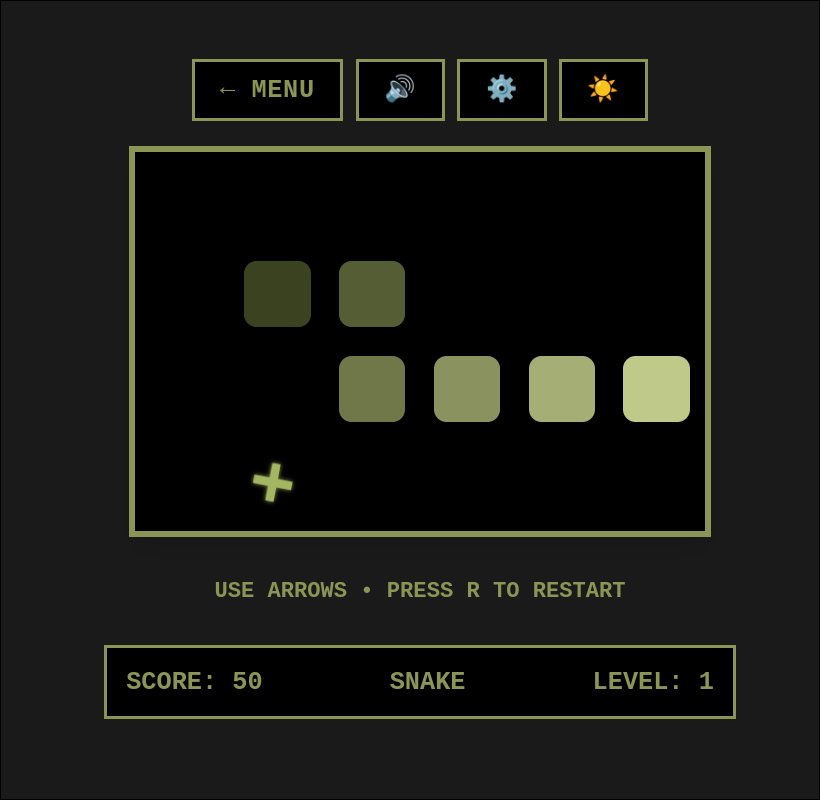
\includegraphics[width=\textwidth]{../screenshots/playing.png}
\end{columns}
\end{frame}

%------------------------------------------------
\begin{frame}{Why Is This Non-Trivial?}
\begin{itemize}
  \item Despite simplicity, the state space is \textbf{huge}
  \item For a 20×20 grid:
  \begin{itemize}
    \item 400 possible positions per segment
    \item Snake length varies from 1 to 400
    \item Direction: 4 choices
    \item Food placement: 399 positions
  \end{itemize}
  \item \textbf{Cannot} store or explore all states exhaustively
\end{itemize}

\vspace{0.3cm}
\begin{block}{Solution}
Rely on \textbf{state invariants} and \textbf{inductive reasoning}
\end{block}
\end{frame}

%------------------------------------------------
\begin{frame}{Our Approach}
\begin{enumerate}
  \item Implemented visual frontend for understanding game behavior
  \item Coded backend in Scala
  \item Ported to Stainless with verification annotations
  \item Integrated invariants into state transition logic
  \item Verified that transitions preserve invariants
\end{enumerate}

% \vspace{0.5cm}
% \begin{block}{Key Technique}
% THIS IS WRONG!
% Introduce a single \textbf{invalid state} reachable only if an invariant is violated
% \end{block}
\end{frame}


%================================================
% REMAINING 10 MINUTES
%================================================

%------------------------------------------------
\begin{frame}{State Machine Model}
\centering
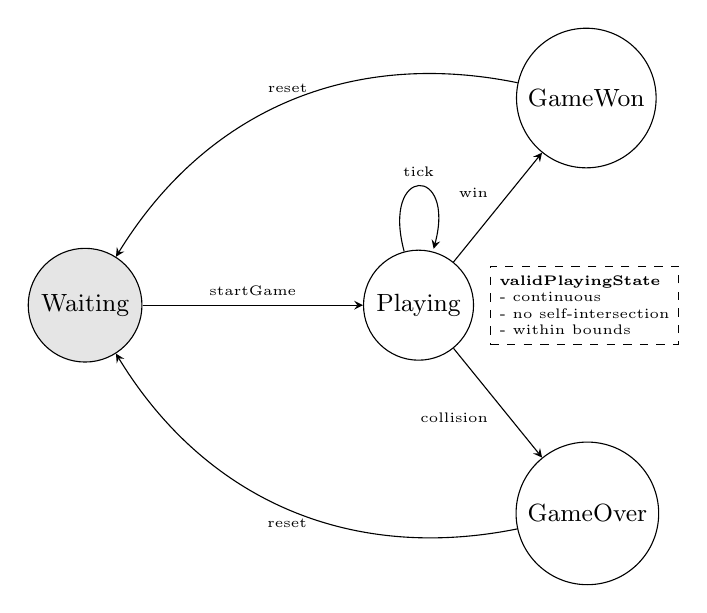
\begin{tikzpicture}[
    ->,
    >=stealth,
    node distance=2.8cm,
    state/.style={circle, draw, minimum size=1.2cm, font=\small},
    initial/.style={state, fill=gray!20}
]

\node[initial] (waiting) {Waiting};
\node[state] (playing) [right=of waiting] {Playing};
\node[state] (gameover) [below right=1.5cm and 1cm of playing] {GameOver};
\node[state] (gamewon) [above right=1.5cm and 1cm of playing] {GameWon};

\path
    (waiting) edge node[above, font=\tiny] {startGame} (playing)
    (playing) edge[loop above] node[above, font=\tiny] {tick} (playing)
    (playing) edge node[below left, font=\tiny] {collision} (gameover)
    (playing) edge node[above left, font=\tiny] {win} (gamewon)
    (gameover) edge[bend left=35] node[below, font=\tiny] {reset} (waiting)
    (gamewon) edge[bend right=35] node[above, font=\tiny] {reset} (waiting);

\node[draw, rectangle, dashed, align=left, font=\tiny, right=0.2cm of playing] {
  \textbf{validPlayingState}\\
  - continuous\\
  - no self-intersection\\
  - within bounds
};

\end{tikzpicture}

\textbf{Invariant:} A property that holds in all reachable valid states
\end{frame}

%------------------------------------------------
\begin{frame}[fragile]{Data Structures}
\begin{flushright}
\tiny\textcolor{gray}{GameState.scala, Invariants.scala}
\end{flushright}
\vspace{-0.5cm}
\begin{lstlisting}[style=scala]
case class Position(x: BigInt, y: BigInt)

case class GameState(
  snake: List[Position],        // Head at front
  food: Option[Position],
  direction: Direction,
  status: GameStatus,
  ...
)

def validPlayingState(s: GameState): Boolean =
  s.status == Playing &&
  0 < s.snake.length && 
  s.snake.length < s.gridWidth * s.gridHeight &&
  withinBounds(s.snake, s.gridWidth, s.gridHeight) &&
  noSelfIntersection(s.snake) &&
  continuous(s.snake)
\end{lstlisting}
\end{frame}

\begin{frame}[fragile]{Game Logic}
\begin{lstlisting}[style=scala]
def initializeGame(state: GameState, ...): GameState = {
  ...
}.ensuring(validPlayingState(_))


def processGameTick(state: GameState, ...): GameState = {
  require(validPlayingState(state))
  ...
  if state.hasCollision(newHead) then
    currState.copy(status = GameStatus.GameOver, ...)
  ...
  val newTail =
     if ateFood then currState.snake
     else withoutLast(currState.snake)
  val newSnake = newHead :: newTail
  val hasWon = newSnake.length == currState.gridWidth * currState.gridHeight
  ...
}.ensuring(res =>
    res.status == GameStatus.Playing ==> validPlayingState(res)
)

\end{lstlisting}
\end{frame}
%------------------------------------------------
\begin{frame}[fragile]{Property 1: Continuity}
\textbf{Challenge:} Initial implementation used numeric recursion (\texttt{take(n)})

Stainless struggled with numeric counters!

\vspace{0.3cm}
\textbf{Solution:} Rewrite with structural recursion:

\begin{flushright}
\tiny\textcolor{gray}{Invariants.scala}
\end{flushright}
\vspace{-0.5cm}
\begin{lstlisting}[style=scala]
def continuous(snake: List[Position]): Boolean =
  snake match
    case Cons(h1, Cons(h2, t)) => 
      adjacent(h1, h2) && continuous(Cons(h2, t))
    case _ => true

def adjacent(a: Position, b: Position): Boolean =
  (a.x == b.x && abs(a.y - b.y) == 1) ||
  (a.y == b.y && abs(a.x - b.x) == 1)
\end{lstlisting}

\textbf{Result:} Stainless can reason about this via structural induction
\end{frame}

%------------------------------------------------
\begin{frame}[fragile]{Property 2: Within Bounds}
\begin{flushright}
\tiny\textcolor{gray}{Invariants.scala}
\end{flushright}
\vspace{-0.5cm}
\begin{lstlisting}[style=scala]
def withinBounds(
  snake: List[Position],
  width: BigInt,
  height: BigInt
): Boolean =
  snake.forall(p => 
    0 <= p.x && p.x < width && 
    0 <= p.y && p.y < height
  )
\end{lstlisting}

\vspace{0.3cm}
\textbf{Challenge:} Prove that removing tail preserves this property

\begin{lstlisting}[style=scala]
def withoutLastWithinBounds(@induct s: List[Position], 
                            width: BigInt,
                            height: BigInt): Unit = {
  require(withinBounds(s, width, height))
}.ensuring(withinBounds(withoutLast(s), width, height))
\end{lstlisting}
\end{frame}

%------------------------------------------------
\begin{frame}[fragile]{Property 3: No Self-Intersection}
\begin{flushright}
\tiny\textcolor{gray}{Invariants.scala}
\end{flushright}
\vspace{-0.5cm}
\begin{lstlisting}[style=scala]
def noSelfIntersection(snake: List[Position]): Boolean =
  ListSpecs.noDuplicate(snake)
\end{lstlisting}

\vspace{0.3cm}
\textbf{Challenges:}
\begin{itemize}
  \item Proving list uniqueness is preserved
  \item Required multiple helper lemmas about list operations:
  \begin{itemize}
    \item \texttt{withoutLastIsSubseq}: Removing the last element gives a subsequence
    \item \texttt{noDuplicateSubseq}: From \texttt{ListSpecs}
    \item \texttt{subseqNotContains}: From \texttt{ListSpecs}, snake doesn't contain \texttt{newHead}, therefore, \textttt{withoutLast(snake)} doesn't.
  \end{itemize}
\end{itemize}

\vspace{0.3cm}
\begin{lstlisting}[style=scala]
def withoutLastNoSelfIntersection(s: List[Position]): Unit = {
  require(noSelfIntersection(s))
  withoutLastIsSubseq(s)
  ListSpecs.noDuplicateSubseq(withoutLast(s), s)
}.ensuring(noSelfIntersection(withoutLast(s)))
\end{lstlisting}
\end{frame}

%------------------------------------------------
\begin{frame}[fragile]{Grid Generation Challenge}
\textbf{Problem:} Prove grid has no duplicate positions and always has space

\begin{flushright}
\tiny\textcolor{gray}{GameLogic.scala}
\end{flushright}
\vspace{-0.5cm}
\begin{lstlisting}[style=scala]
def grid(width: BigInt, height: BigInt): List[Position] = {
  require(width > 0 && height > 0)
  range(width * height).map(i => 
    Position(i % width, i / width)
  )
}.ensuring(_.length == width * height)
\end{lstlisting}

\textbf{Proof strategy:}
\begin{enumerate}
  \item Prove \texttt{range(n)} generates unique integers
  \item Prove mapping $i \mapsto Position(i \bmod w, i \div w)$ is bijective
  \item Compose to show grid has no duplicates
\end{enumerate}

\begin{lstlisting}[style=scala]
def gridNoDuplicate(width: BigInt, height: BigInt): Unit = {
  require(width > 0 && height > 0)
  rangeNoDuplicate(width * height, 0)
  gridBijectionNoDuplicate(range(width * height), width)
}.ensuring(ListSpecs.noDuplicate(grid(width, height)))
\end{lstlisting}
\end{frame}
%------------------------------------------------
\begin{frame}[fragile]{Food Generation Safety}
\textbf{Requirement:} Food must never spawn on snake

\begin{flushright}
\tiny\textcolor{gray}{GameLogic.scala}
\end{flushright}
\vspace{-0.5cm}
\begin{lstlisting}[style=scala]
def generateFood(state: GameState, seed: BigInt): Position = {
  require(validPlayingState(state))
  
  val emptyPositions = 
    grid(state.gridWidth, state.gridHeight) -- state.snake
  gridWithoutSnakeNonEmpty(state)  // Proves nonEmpty
  val index = abs(seed) % emptyPositions.length
  
  emptyPositions(index)
}.ensuring(!state.snake.contains(_))
\end{lstlisting}

\vspace{0.3cm}
\textbf{Key lemma:}
\begin{lstlisting}[style=scala]
def noDuplicateFilterLength[T](l1: List[T], l2: List[T]): Unit = {
  require(ListSpecs.noDuplicate(l2) && l1.length < l2.length)
}.ensuring((l2 -- l1).length >= l2.length - l1.length)
\end{lstlisting}
\end{frame}


%------------------------------------------------
\begin{frame}{Verification Results}
\begin{columns}[c]
\begin{column}{0.55\textwidth}
\centering
\begin{tabular}{|l|c|}
\hline
\textbf{Metric} & \textbf{Value} \\
\hline
Total verification conditions & 184 \\
Valid & 184 \\
Invalid & 0 \\
Unknown & 0 \\
\hline
Verification time & 4.56s \\
Functions verified & 82 \\
\hline
\end{tabular}
\end{column}
\begin{column}{0.4\textwidth}
\centering
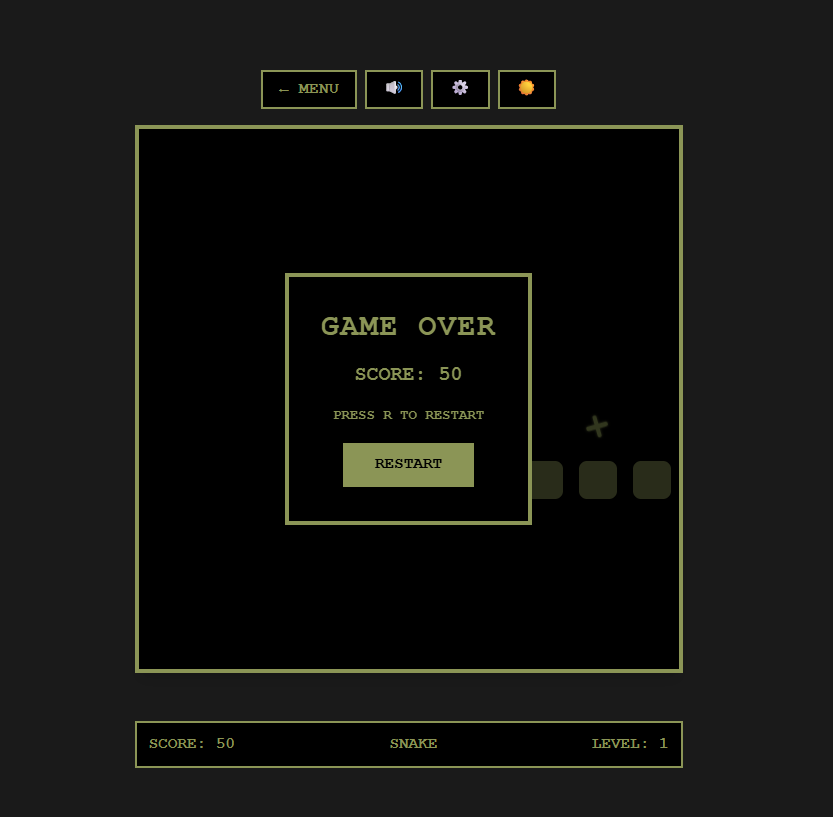
\includegraphics[width=1\textwidth]{../screenshots/gameover.png}
\end{column}
\end{columns}
\end{frame}

%------------------------------------------------
\begin{frame}{What Remains To Be Done}
\begin{itemize}
  \item \textbf{Additional properties:}
  \begin{itemize}
    \item Snake length monotonicity (grows only by 1)
    \item Win condition correctness formal proof
  \end{itemize}
  
  \item \textbf{Extended verification:}
  \begin{itemize}
    \item Direction queueing correctness (partially done)
    \item Food always within bounds
  \end{itemize}
  
  \item \textbf{Game variants:}
  \begin{itemize}
    \item Multiple food items
    \item Obstacles on the board
    \item Teleporting borders
  \end{itemize}
\end{itemize}
\end{frame}

%------------------------------------------------
\begin{frame}{Summary}
\textbf{What we accomplished:}
\begin{itemize}
  \item Formally verified 3 core safety properties of Snake
  \item Proved impossibility of key bugs (when state is valid):
  \begin{itemize}
    \item Out-of-bounds access
    \item Self-collision
    \item Discontinuous snake
  \end{itemize}
  \item Demonstrated practical workflow with Stainless
  \item Integrated verification into CI/CD pipeline
\end{itemize}

\vspace{0.5cm}
\textbf{Key lessons:}
\begin{itemize}
  \item Structural recursion >> numeric recursion for Stainless
  \item Helper lemmas are essential to guide SMT solver
  \item Invariant design is critical for provability
\end{itemize}
\end{frame}

%------------------------------------------------
\begin{frame}
\centering
\Huge Thank You!

\vspace{1cm}
\Large Questions?

\vspace{1cm}
\normalsize
Repository: \texttt{github.com/mohamedtahaguelzim/formal-snake}
\end{frame}

\end{document}

